\section{Calibration}

The calibration of the LTCC detector consisted of matching the gains of the 216 PMTs. The main reason for this
is that the FADC250 thresholds and sampling acquisition parameters are the same for all channels.

This gain calibration was carried out by using data with an electron beam incident on the experiment target. A
random trigger was saved in the data stream at a rate of 100~Hz. This data subset includes LTCC events with
PMT noise above the FADC pedestal, containing the single photo-electron signal (SPE).

At the beginning of each experiment the PMT high voltages are adjusted to align the peak positions to a particular
ADC value of $ADC_{SPE} = 200$. An example of the gain matching is shown in \F{gainMatching}. The ADC spectra
(see for \F{speCalibration} for typical histograms) were fit to identify the SPE peak positions.

During analysis of physics events, the reconstructed number of photo-electrons for the digitized ADC value is
calculated to be ADC/$ADC_{SPE}$. It was found that the gains of several of the photo-tubes drifted with time, so
the calibration procedure was repeated every week to ensure that the values of $ADC_{SPE}$ reflect the latest
gains and that these variations do not affect the LTCC response.

\begin{figure}[H]
	\centering
	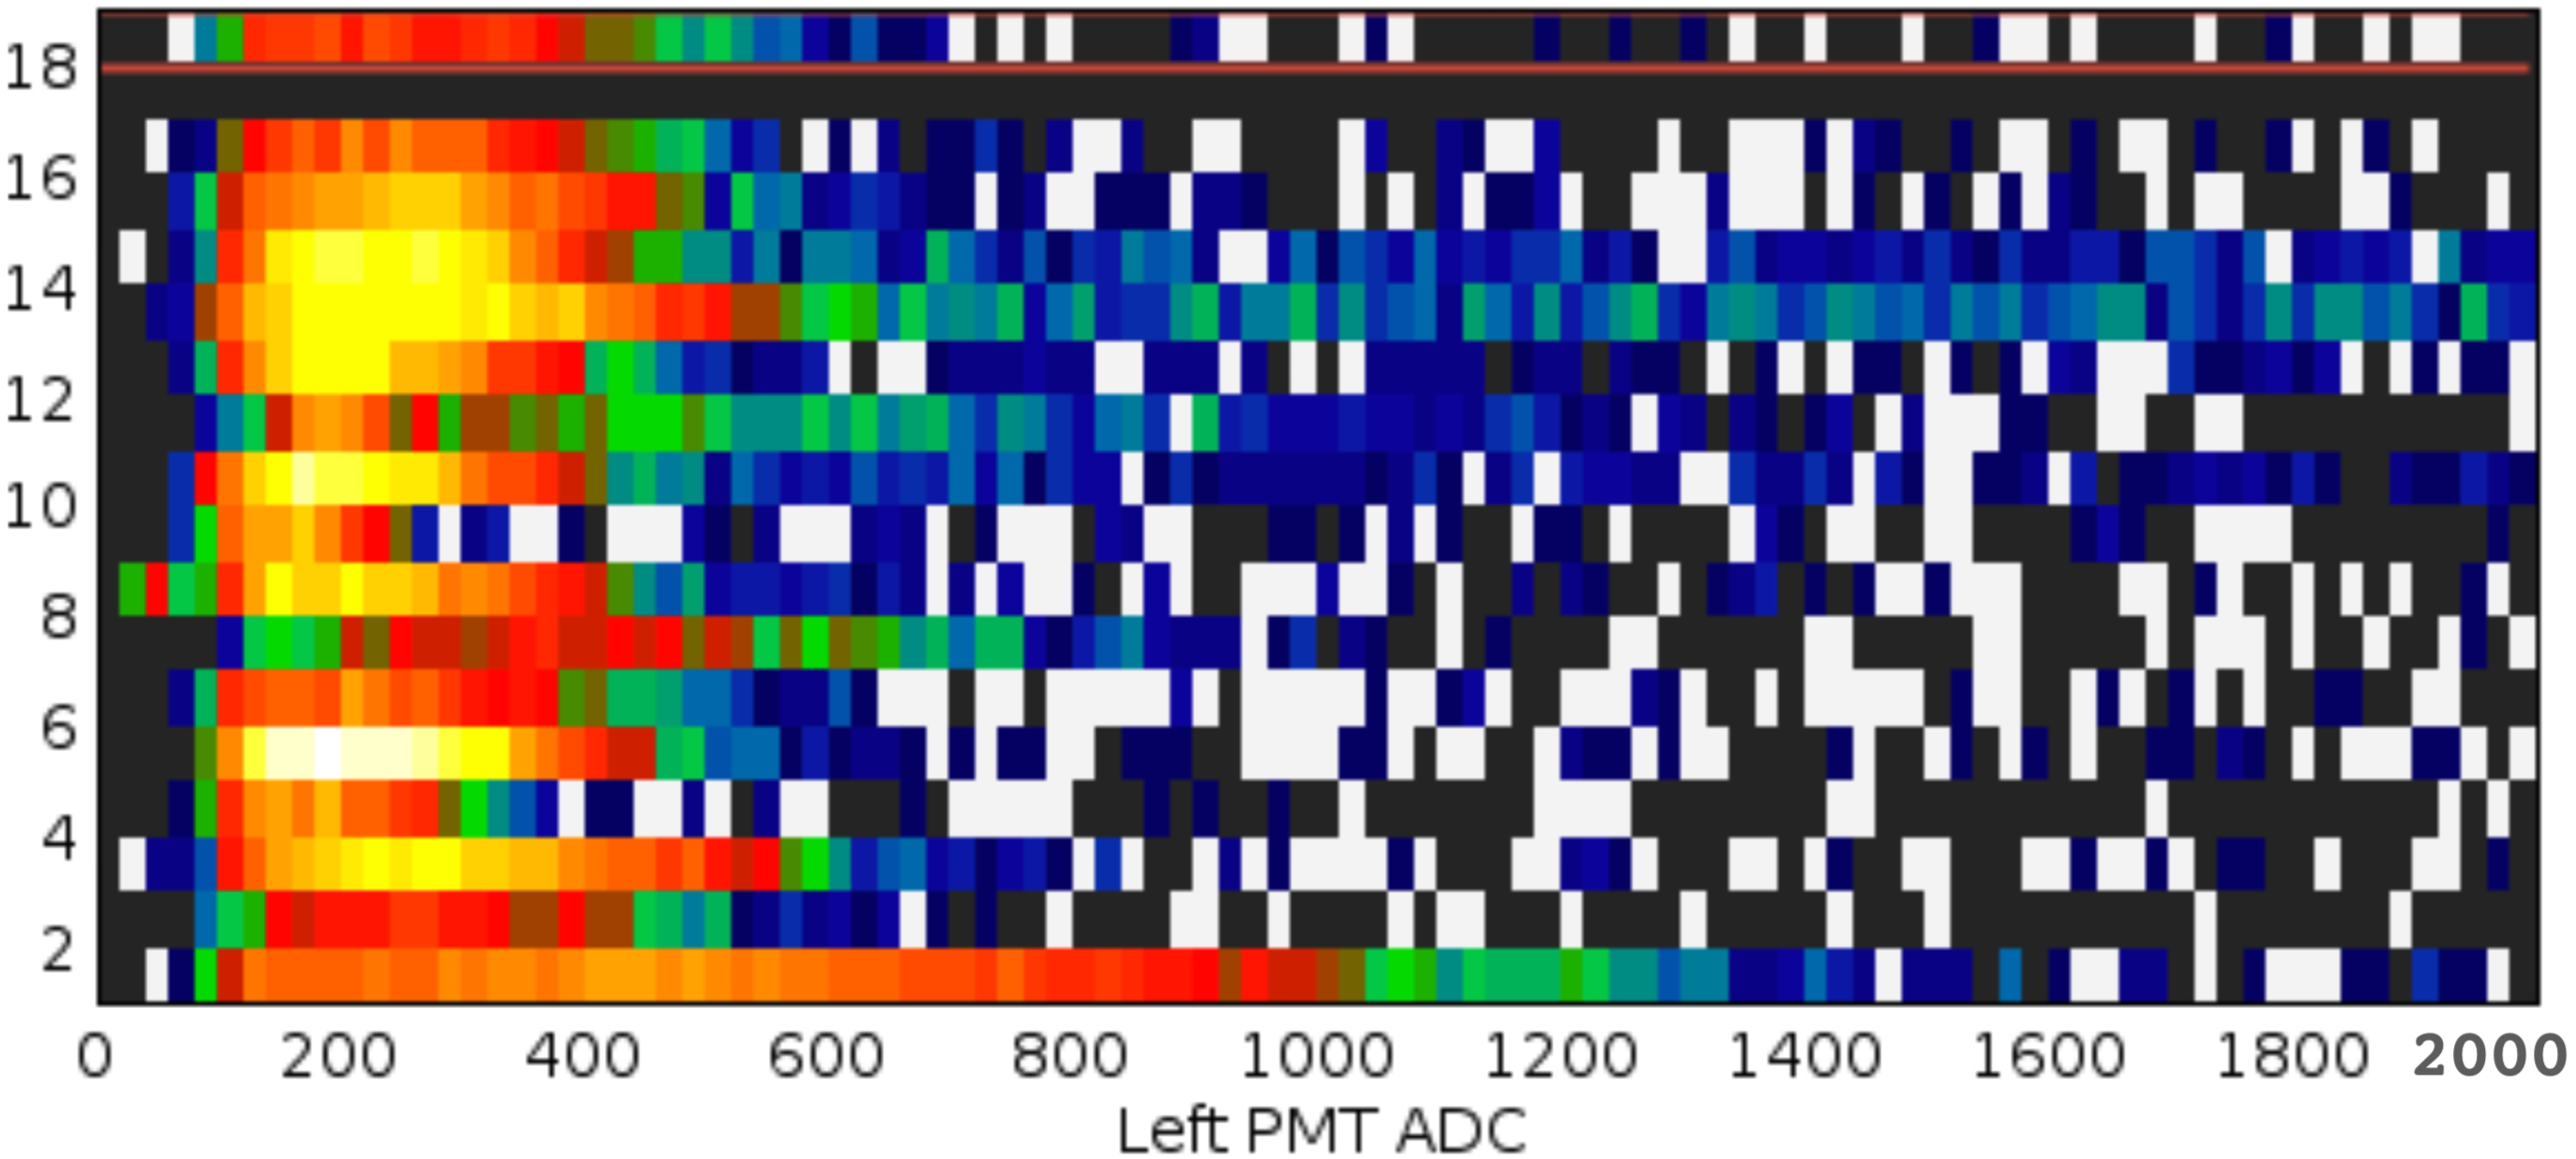
\includegraphics[width=1.05\columnwidth, keepaspectratio]{img/gainMatchingBefore.png}
	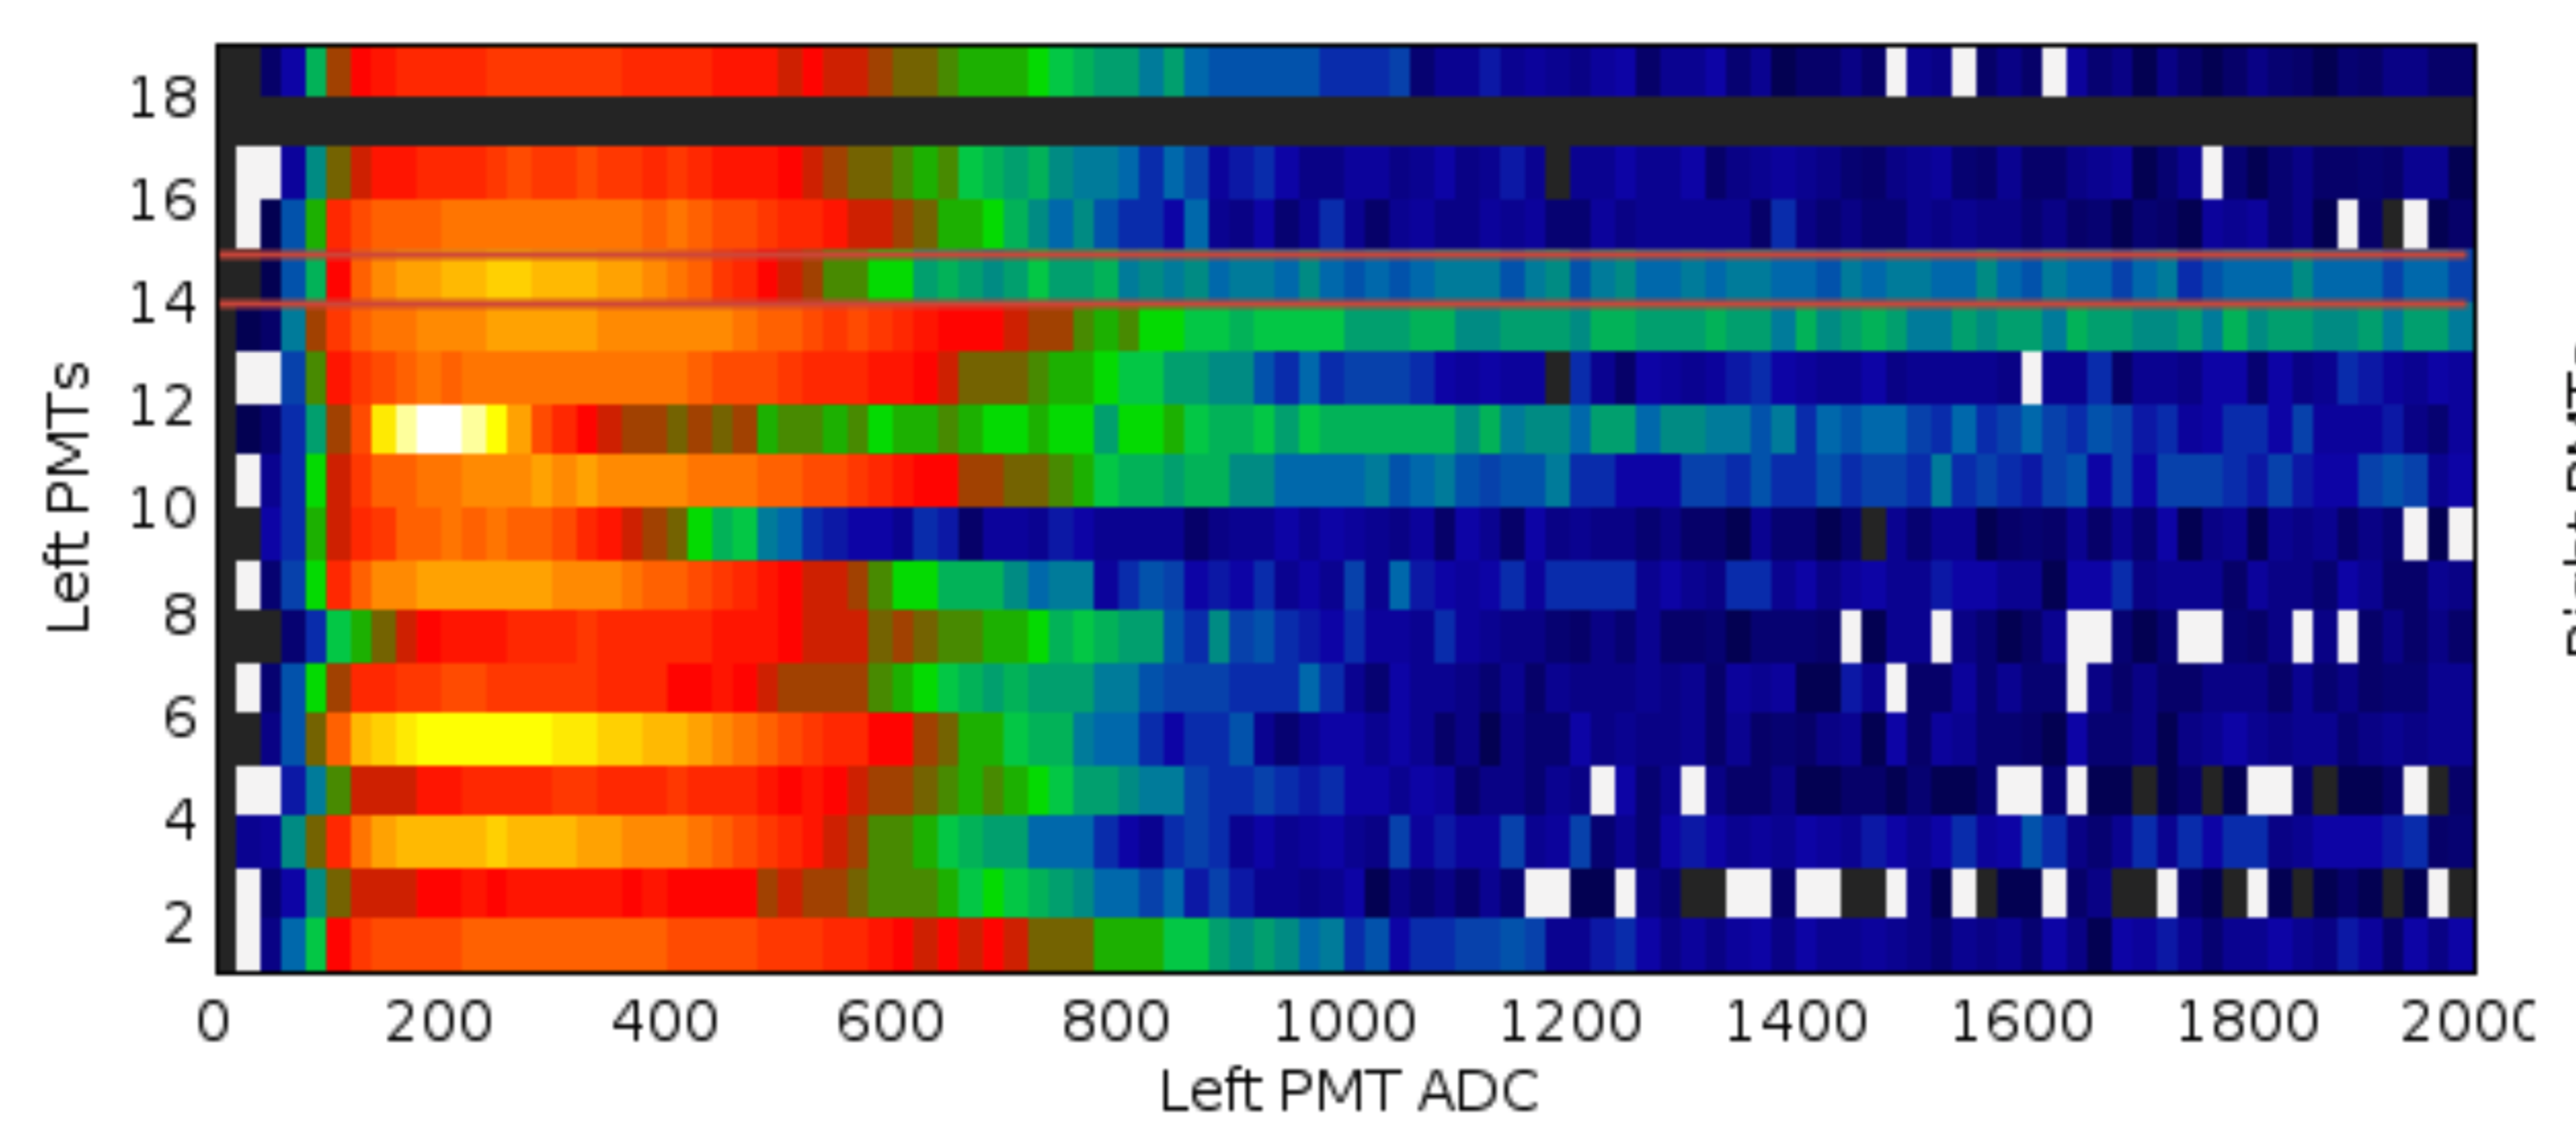
\includegraphics[width=1.05\columnwidth, keepaspectratio]{img/gainMatchingAfter.png}
	\caption{Plot of PMT number vs. ADC for the LTCC sector 3 right side PMTs. Data is from the first production
          run in spring 2018. Top: before gain matching several channels do not show a SPE peak position at
          $ADC_{SPE} = 200$. Bottom: after gain matching the PMT responses are well aligned.}
	\label{fig:gainMatching}
\end{figure}

\begin{figure*}
	\centering
	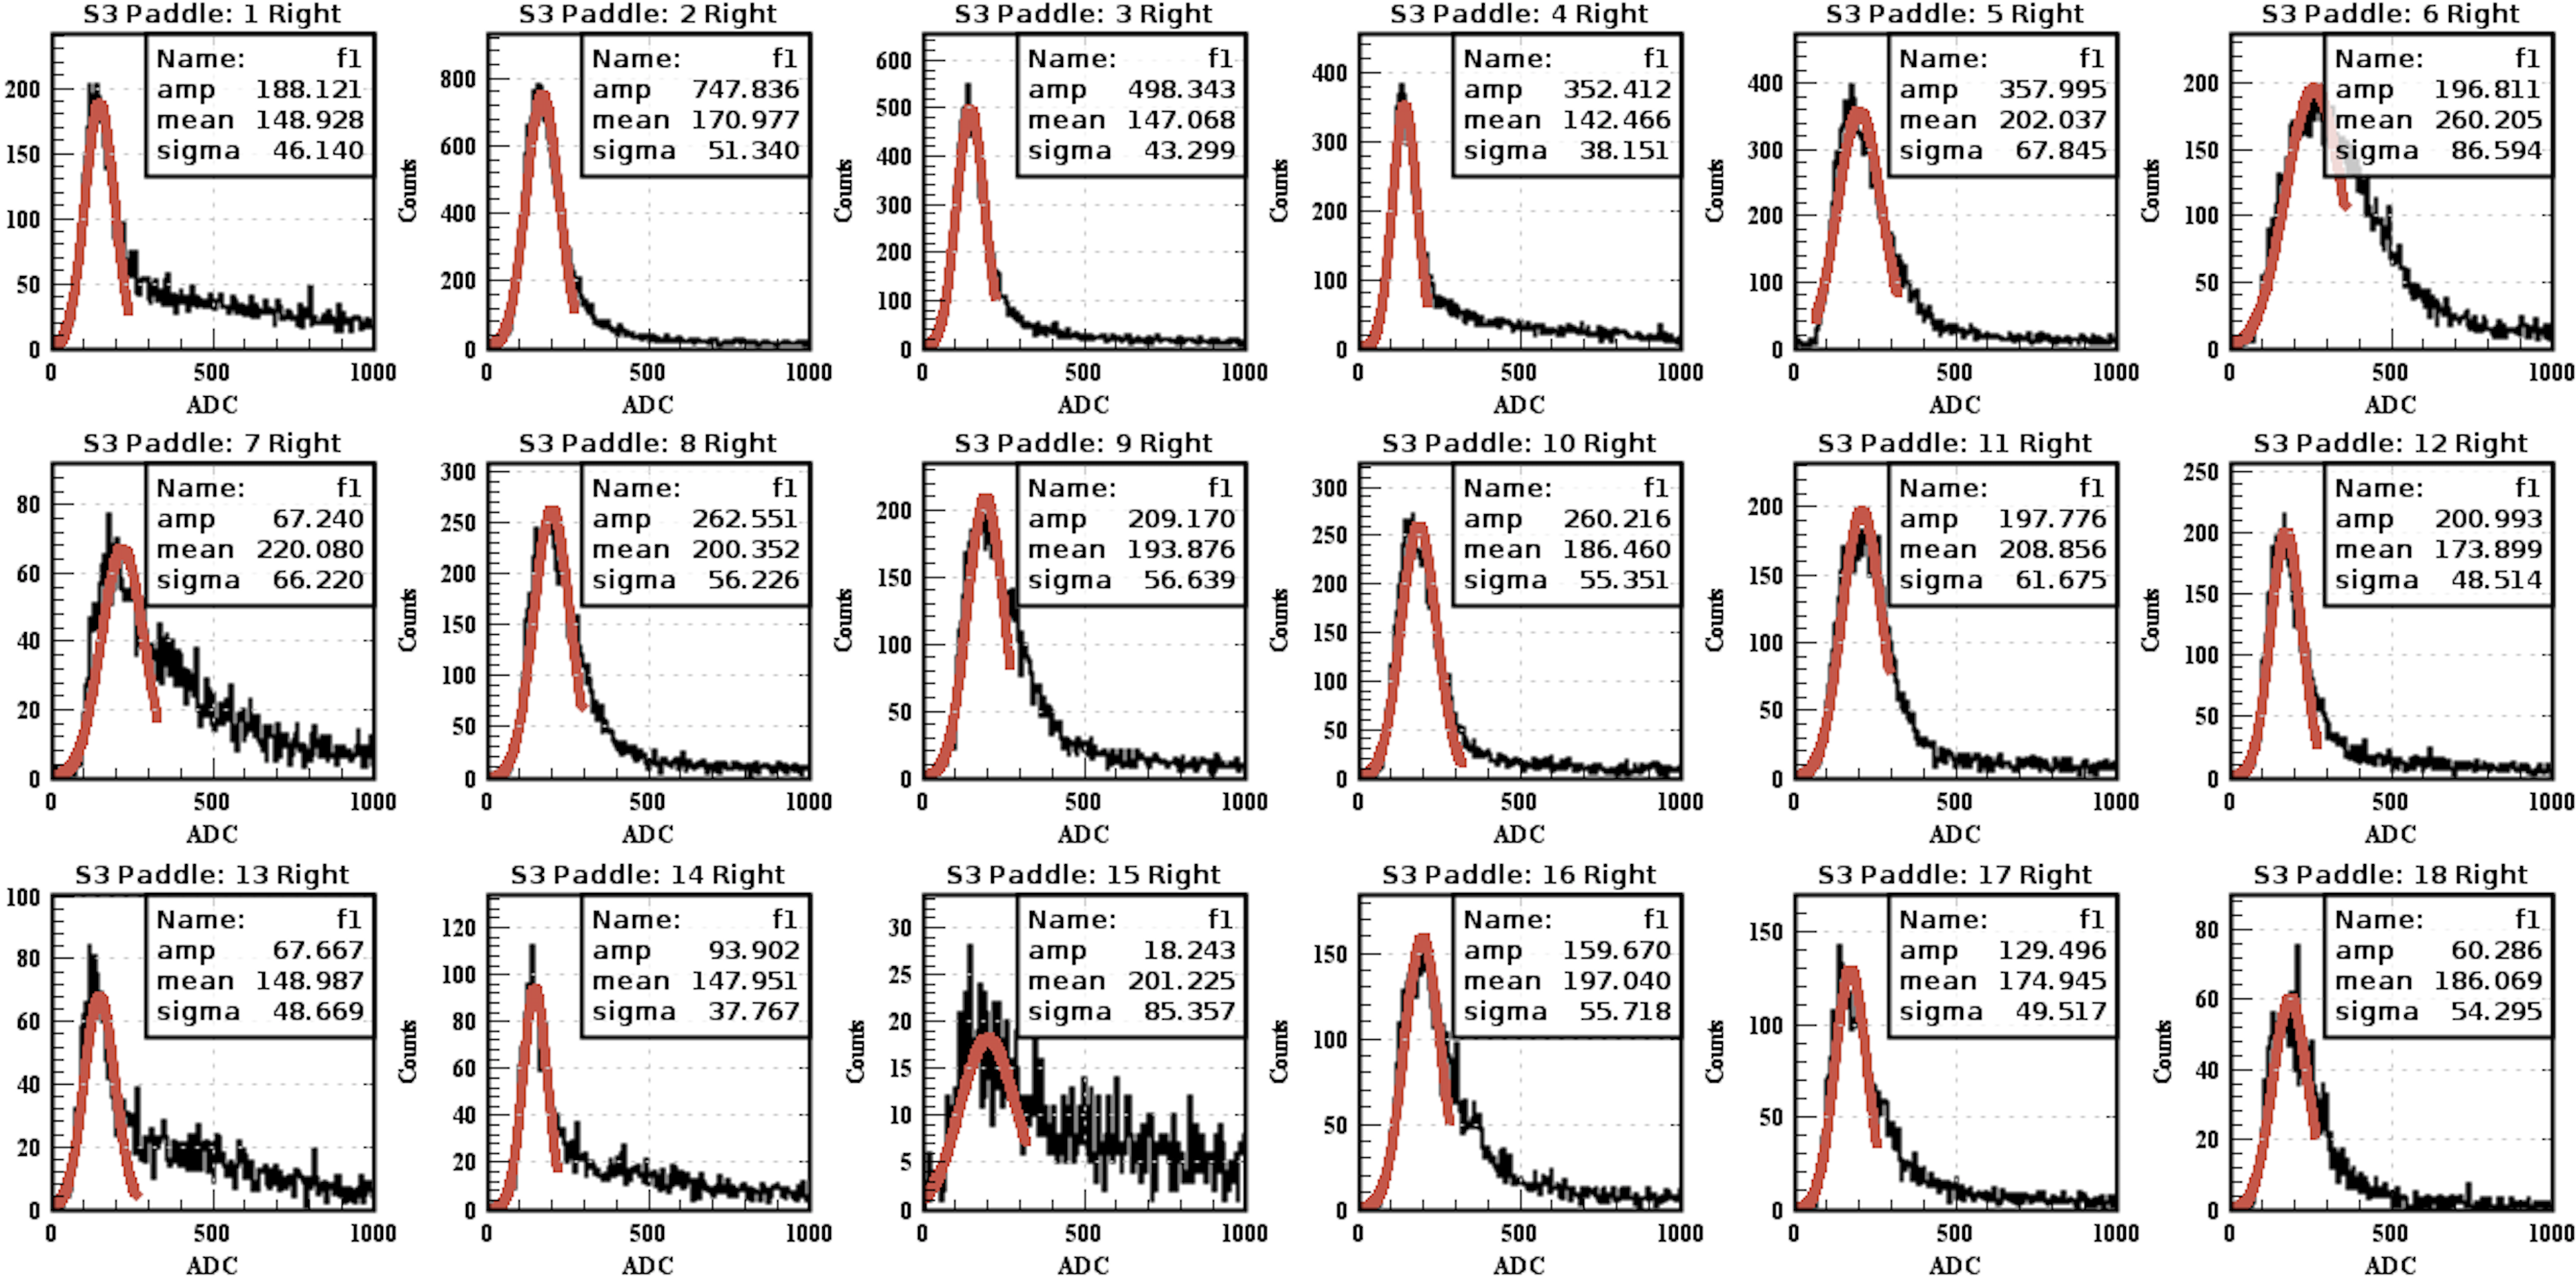
\includegraphics[width=2.1\columnwidth,keepaspectratio]{img/spe.png}
	\caption{The LTCC sector 3 right side ADC spectra. Data is from the first production run in spring 2018.
          The SPE peak positions are fit with a Gaussian function and the mean $ADC_{SPE}$ parameters are recorded
          in the calibration database. The reconstructed number of photo-electrons for the digitized ADC value is
          then ADC/$ADC_{SPE}$. Some anomalous PMTs can be seen: \#6 shows a larger than normal width (HV too large)
          and \# 15 shows a smaller than normal signal to width ratio, probably due to PMT hardware problems.}
	\label{fig:speCalibration}
\end{figure*}
